\section{Passwörter}
\begin{frame}{Passwörter}
  \begin{itemize}
    \item<+->{Wer hat mindestens fünf Online-Accounts?}
    \item<+->{Wer hat dafür mindestens drei verschiedene Passwörter?}
    \item<+->{Wer beachtet, Passwörter nur auf der echten Website einzugeben?}
  \end{itemize}
\end{frame}

\begin{frame}{Anzahl Passwörter}
  \begin{itemize}
    \item Zugangsdaten werden bei Hackerangriffen auf Diensteanbieter gestohlen
    \begin{itemize}
      \item Angreifer probieren Zugangsdaten auch anderswo
      \item Schaden lässt sich begrenzen, wenn Benutzername und Passwort nur bei diesem einen Anbieter passen
    \end{itemize}
    \item Besonders wichtig: E-Mail-Accounts
    \begin{itemize}
      \item Weil ,,Passwort zurücksetzen`` oft via E-Mail
      \item Wer den E-Mail Account übernommen hat,\\ kann dadurch sämtliche Accounts übernehmen
    \end{itemize}
    \item Ideal: Für jeden Anbieter anderes Passwort
    \item Alternative: Passwörter ,,salzen``
    \begin{itemize}
      \item \textit{passwort}.amz für Onlineshop a
      \item \textit{passwort}.zal für Onlineshop z
      \item \textit{anderespasswort} für Mails
    \end{itemize}
  \end{itemize}
\end{frame}

\begin{frame}{Passwort Wiederverwertung}
  \begin{center}
    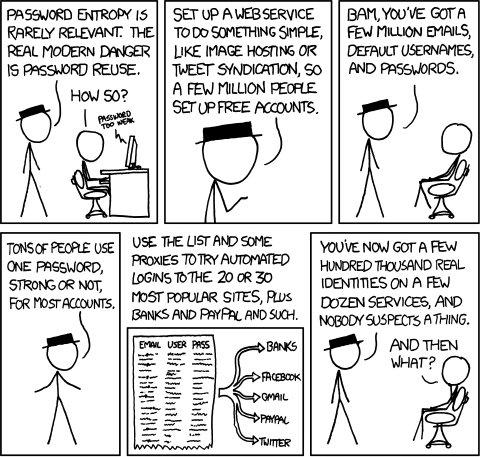
\includegraphics[height=0.8\textheight]{images/password_reuse_top.png}\\
  \end{center}
  \tiny Bildquelle: Ausschnitt aus \href{http://xkcd.com/792/}{xkcd: Password Reuse / CC BY-NC 2.5}
\end{frame}

\begin{frame}{Sichere Passwörter}
  \begin{block}{Anforderungen}
  \begin{itemize}
    \item Klein- und Großbuchstaben, Zahlen,\\ begrenzt: Sonderzeichen
    \item Wichtiger: Lang genug!
  \end{itemize}
  \end{block}
  \begin{block}{Merkbarkeit}
  \begin{itemize}
    \item Pass\emph{satz} statt Passwort\\
      Beispiel: \texttt{margaretthatcheris110\%SEXY}\\
      {\scriptsize (aus Snowden-Interview: \url{https://www.youtube.com/watch?v=yzGzB-yYKcc})}
    \item würfeln, dann sieben zufällige Wörter verwenden\\
      {\scriptsize siehe \url{https://theintercept.com/2015/03/26/passphrases-can-memorize-attackers-cant-guess/}}
  \end{itemize}
  \end{block}
\end{frame}

\begin{frame}{Passwort-Manager}
  \begin{itemize}
    \item Verwalten Passwörter in verschlüsselter Datenbank
    \item Nutzer muss sich nur Datenbankpasswort merken
  \end{itemize}

  \begin{columns}[T]
    \begin{column}{.45\textwidth}
      \pause
      \begin{blit}{Vorteile}
        \small
        \item Erzeugt deutlich bessere Passwörter als Durchschnittsmensch
        \item Erleichtert es,\\jedes Passwort nur\\einmal zu verwenden
      \end{blit}
    \end{column}
    \begin{column}{.55\textwidth}
      \pause
      \begin{blit}{Nachteil}
        \small
        \item Eingefangene Schadsoftware\\bekommt möglicherweise\\alle Passwörter auf einmal\\
          \emph{Aber:\\ Schadsoftware kann auch ohne Passwort-Manager alle Tastatureingaben mitlesen}
      \end{blit}
    \end{column}
  \end{columns}
  \pause
  \begin{blit}{Anmerkungen}
    \small
    \item Entscheidung zwischen lokalen und \glqq Cloud\grqq -Datenbanken\\ = \glqq klassischer\grqq\ Tradeoff zwischen Sicherheit und Komfort
    \item Backups! -- und wichtige Passwörter trotzdem merken!
    \item Unsere Empfehlung: KeePass(X)
  \end{blit}
\end{frame}

\endinput
